\section{Ziel}
Es soll der Interferenzkontrast eines Sagnac-Interferometers ermittelt werden.
Außerdem soll mit Hilfe des Sagnac-Interferometers der Brechungsindex von Glas
bzw. Luft ermitelt werden.

\section{Theorie}
\subsection{Sagnac-Interferometer}
\label{sec:SI}

In Abbildung \ref{fig:sagnac} wird der Versuchsaufbau des Sagnac-Interferometers
dargestellt.

\begin{figure}[H]
  \centering
  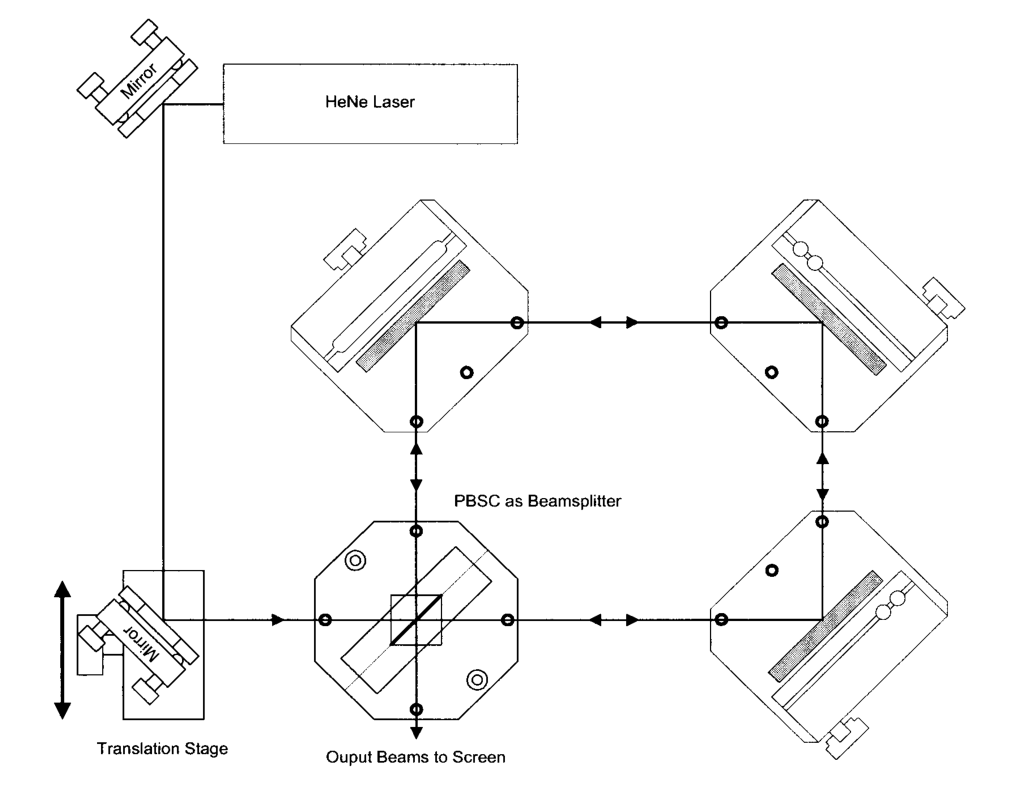
\includegraphics
  [width=12cm]{sagnac.png}
  \caption{Versuchsaufbau des Sagnac-Interferometers.}
  \label{fig:sagnac}
  \cite{skript}
\end{figure}

Es wird ein HeNe-Laser verwendet, welcher an zwei Spiegeln reflektiert wird und
über ein PBSC (Polarizing Beam-Splitter Cube) in zwei Teilstrahlen aufgeteilt wird.
Die Laserstrahlen werden in entgegengesetzter Richtung an drei Spiegeln im Rechteck
reflektiert und treffen wieder auf den PBSC.
Beide Strahlen legen einen näherungsweise gleichen Weg zurück.
Dort laufen die Teilstrahlen wieder zusammen, welche miteinander interferieren sollen.

Da die zusammenlaufenden Laserstrahlen genau senkrecht aufeinander linear polarisiert
sind, können keine Interferenzen stattfinden.
Daher muss der Strahl erneut in seine Komponenten aufgeteilt werden, um diesen
auszuwerten.
Hierzu wird, wie in Abbildung \ref{fig:separator} dargestellt, ein PBSC verwendet, der um einen 45° Winkel gekippt ist.
Die beiden Teilstrahlen treffen auf jeweils eine Diode.
Die Intensitäten werden als Spannungen auf einem Oszilloskop dargestellt und interpretiert.

\begin{figure}[H]
  \centering
  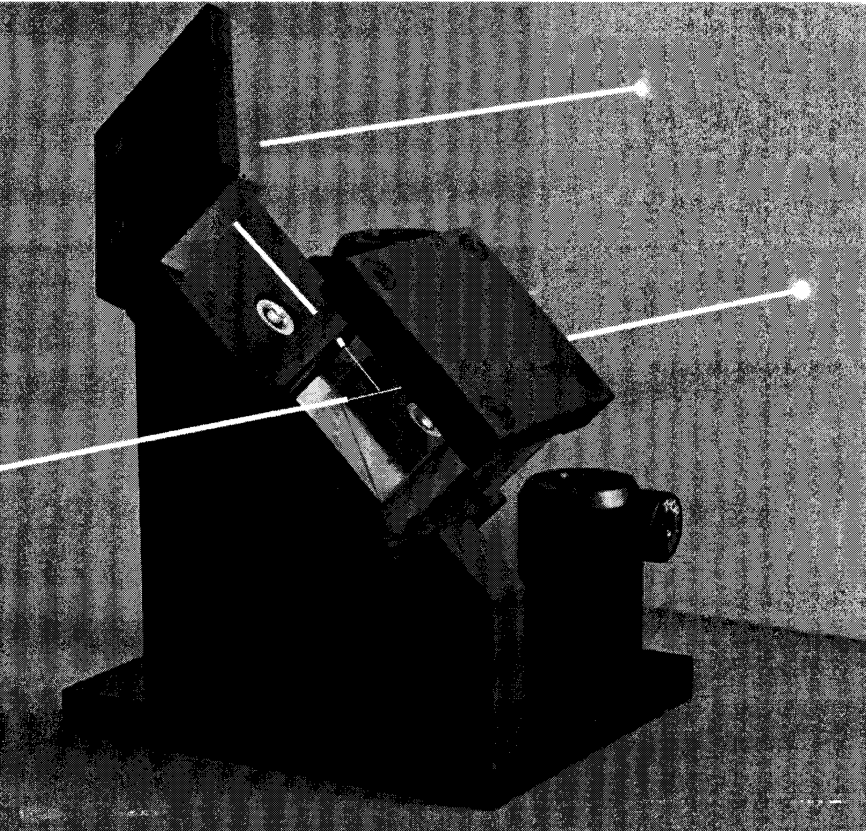
\includegraphics
  [width=10cm]{separator.png}
  \caption{Nutzung des PBSC als Polarisationstrenner.}
  \label{fig:separator}
  \cite{skript}
\end{figure}

\subsection{Der Interferenzkontrast und Lichtintensität}

Der Interferenzkontrast ist abhängig von der Lichtintensität je nach Polarisationsrichtung.
Der Kontrast ist definiert als
\begin{equation}
  K := \frac{I_{max} - I_{min}}{I_{max} + I_{min}}.
  \label{eqn:kontrast}
\end{equation}
Bei Unkenntlichkeit beträgt dieser Null ($I_{max} = I_{min}$) und im Idealfall gilt $K=1$.

Für die Anteile des Strahls gilt
\begin{gather*}
  E_1 = E_0\cos(\phi)\cos(\omega t) \\
  E_2 = E_0\sin(\phi)\cos(\omega t + \delta),
\end{gather*}
wobei $\delta$ die relative Phasenverschiebung der Teilwellen zueinander beschreibt.
Für die Intensität der überlagerten Strahlen gilt
\begin{equation*}
  I \propto <|E_1 + E_2|>.
\end{equation*}
Durch Einsetzen und durch ausnutzen der Relationen
\begin{gather*}
  <\cos^2(\alpha x + y)> = \frac{1}{2} \\
  \delta = 2\pi n , \, n\in\mathrm{N}_0,\, \text{für konstriktive Interferenz und} \\
  \delta = (2n+2)\pi,\, n\in\mathrm{N}_0,\, \text{für destruktive Interferenz}
\end{gather*}
folgt nach Umformung für konstruktive bzw. destruktive Interferenz
\begin{equation*}
  I_{max/min} \propto \frac{1}{2}E_0^2 (1 \pm 2\cos(\phi)\sin(\phi))
\end{equation*}
bzw.
\begin{equation}
  I_{max/min} \propto I_0(1 \pm 2\cos(\phi)\sin(\phi)).
\end{equation}
Es ergibt sich, dass
\begin{align*}
  K \propto |\cos(\phi)\sin(\phi)|.
\end{align*}

\subsection{Brechungsindizes}
Allgemein ist der Brechungsindex definiert als
\begin{equation*}
  n = \frac{c}{v},
\end{equation*}
wobei $c$ die Vakuumlichtgeschwindigkeit und $v$ die Phasengeschwindigkeit des Lichts im Medium ist.
Bei gutem Kontrast kann die Anzahl der Maxima durch die Phasenverschiebung eines
der Strahlen abgezählt werden. Die Phasenverschiebung kann durch eine Gaszelle,
in der der Druck kontinuierlich verändert werden kann, oder durch einen rotierbaren
transparenten Festkörper erzeugt werden.
Allgemein gilt für die Anzahl der Maxima
\begin{equation*}
  M = \frac{\delta}{2\pi},
\end{equation*}
wobei $\delta$ die Phasenverschiebung eines gestörten Strahls gegenüber eines
ungestörten Lichtstrahls angibt.
Der Brechungsindex $n$ von Luft in einer Gaszelle lässt sich mittels der Formel
\begin{equation}
  %n(p_0, T_0) = 1 + \Delta n(p_1,p_2)\frac{T}{T_0}\frac{p_0}{p_2-p_1}
  M = \frac{n-1}{\lambda_{\text{vac}}}(2L)
  \label{eqn:brechluft}
\end{equation}
berechnen,
%wobei $p_0 = 1013,2$mbar und $T_0 = 273,15$K die Standardbedingungen darstellen.
wobei $M$ die Anzahl der Maxima, $\lambda$ die Wellenlänge und $L$ die Länge der Gaszelle ist.

Für den Brechungsindex eines Festkörpers wird eine Halterung für zwei Glasplatten,
die in einem Winkel von $\alpha = 2\cdot\theta_0 = 20°$ zueinander stehen, verwendet.
Allgemein ist Eine Funktion für die Anzahl der Maxima durch eine Glasplatte gegeben durch
\begin{equation}
  M = \frac{T}{\lambda}\cdot\frac{n-1}{2n}\cdot\theta^2.
\label{M_allg}
\end{equation}
Dabei ist $T$ die Dicke der Glasplatte, $\lambda$ die Wellenlänge des Lichts, $n$ der Brechungsindex des Materials und $\theta$ der Rotationswinkel.
Da in diesem Versuch aber zwei Glasscheiben, die in einem relativen Winkel zueinander stehen, verwendet werden,
muss die Formel \eqref{M_allg} über die beiden Winkel $\theta = \theta_0$ und $\theta = -\theta_0$ Taylor-entwickelt werden.
Es ergeben sich
\begin{gather*}
  (\mathcal{T}M)^{(1)}(\theta;\theta_0) = \frac{T}{\lambda}\cdot\frac{n-1}{2n}(\theta^2 + 2\theta_0(\theta-\theta_0)),\\
  (\mathcal{T}M)^{(1)}(\theta;-\theta_0) = \frac{T}{\lambda}\cdot\frac{n-1}{2n}(\theta^2 - 2\theta_0(\theta+\theta_0)).
\end{gather*}
Die Differenz der beiden Entwicklungen liefert
\begin{equation*}
  M_{\mathcal{T}}(\theta) :=
  (\mathcal{T}M)^{(1)}(\theta;\theta_0) - (\mathcal{T}M)^{(1)}(\theta;-\theta_0)
   = \frac{T}{\lambda}\cdot\frac{n-1}{2n}\cdot(4\theta_0\theta)
 \end{equation*}
 Umgestellt nach dem Brechungsindex ergibt sich die Formel,
 mit der sich der Brechungsindex des transparenten Festkörpers berechnen lässt:
\begin{equation}
  n = \frac{-2 \theta_0\theta T}{M\lambda - 2 T\theta\theta_0}.
\label{eqn:glas}
\end{equation}
Hierbei ist $M = M_{\mathcal{T}}(\theta)$.
